\section{Network Protocol and Architecture}

The \oscoin{} network protocol is a realization of the protocol semantics
described in \S~\ref{sec:protocol-semantics}, into the asynchronous network
model.

\subsection{Overview}

The \oscoin{} network is composed of a set of nodes, or \emph{replicas}, which
execute a protocol $\mathcal{P}$. Together, these nodes form a \emph{Replicated
State Machine} with a set of states $\State^*$, a transition function $\apply$,
a starting state $\State_0$, a set of inputs $B_0 \dotso B_n$, and an empty set
of outputs.

% TODO: Are we using the 'P' variable?

Participation in the network protocol is \emph{open} (\ie ``permissionless''),
which makes the replica set dynamic. To achieve consensus in the permissionless
setting, we make use of blockchains~\cite{bitcoin} as the underlying replicated
data-structure, with a method of Sybil resistance such as proof-of-work or
proof-of-stake.  However, unlike other blockchain protocols, we describe a
multi-chain ``block-lattice'' \cite{raiblocks} design with causal consistency
guarantees \cite{causal-consistency} and partial ordering across chains
(Figure~\ref{block-lattice}).

The \oscoin{} protocol can be paired with any blockchain consensus algorithm,
given certain requirements discussed in \S~\ref{consensus}.

\subsection{Block-lattice Architecture}

Block-lattices are a replicated data-structure composed of chains of blocks,
depicted in Figure~\ref{block-lattice}.  Both parallel and synchronized
operations are able to be expressed with this design:  a pair of transactions
on two chains are considered \emph{free}, if they may be processed in parallel,
or \emph{dependent}, if a causal or acausal dependency exists between them.

Each chain in our design functions as a logical unit of organization,
governance, and funding. In other words, each user, organization or community
is expected to operate under their own chain. These individual chains are
called \emph{accounts}. The block-lattice design has numerous advantages for
our use case, including parallel transaction processing, minimal resource
requirements for light clients, instant finality for certain kinds of
transactions, and logical sharding at the account level.

\begin{figure}[!ht]
    \documentclass[tikz]{standalone}

\usetikzlibrary{fit}
\usetikzlibrary{positioning}

\begin{document}
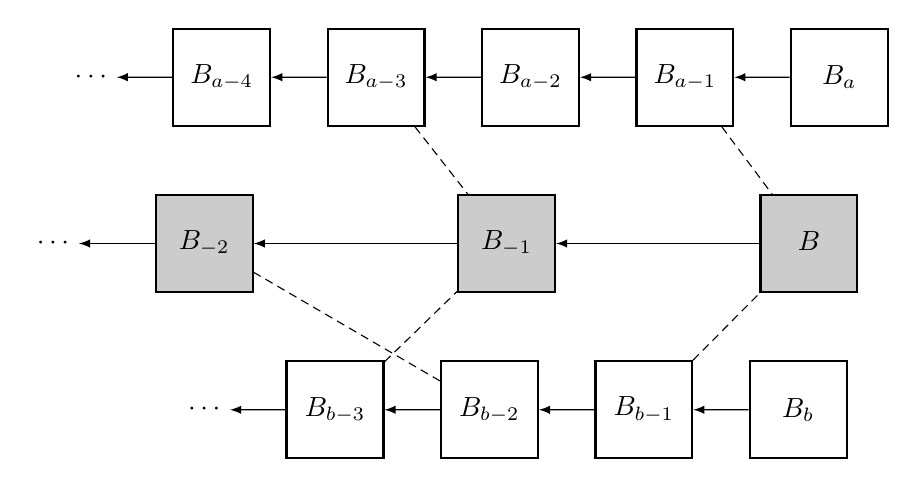
\begin{tikzpicture}[scale=0.96]
    \tikzstyle{root} = [draw=black, thick, fill=black!20, rectangle, minimum height=3.5em, minimum width=3.5em, node distance=3em];
    \tikzstyle{org-block} = [draw, thick, fill=white, rectangle, minimum height=3.5em, minimum width=3.5em, node distance=2em];
    \tikzstyle{link} = [-, thin, densely dashed];
    \tikzstyle{pointer} = [thin, -latex];

    \node (org-a-0) at (-2.5, 2.2)                {$\cdots$};
    \node[org-block] (org-a-1) [right=of org-a-0] {$B_{a-4}$}
        edge [pointer] (org-a-0.east);
    \node[org-block] (org-a-2)  [right=of org-a-1] {$B_{a-3}$}
        edge [pointer] (org-a-1.east);
    \node[org-block] (org-a-3)  [right=of org-a-2] {$B_{a-2}$}
        edge [pointer] (org-a-2.east);
    \node[org-block] (org-a-4)  [right=of org-a-3] {$B_{a-1}$}
        edge [pointer] (org-a-3.east);
    \node[org-block] (org-a-5)  [right=of org-a-4] {$B_{a}$}
        edge [pointer] (org-a-4.east);

    \node (root-0) at (-3, 0)        {$\cdots$};
    \node (root-1) at (-1, 0) [root] {$B_{\rootchain - 2}$}
        edge [pointer] (root-0.east);
    \node (root-2) at ( 3, 0) [root] {$B_{\rootchain - 1}$}
        edge [pointer] (root-1.east);
    \node (root-3) at ( 7, 0) [root] {$B_{\rootchain}$}
        edge [pointer] (root-2.east);

    \node (org-b-0) at (-1, -2.2) {$\cdots$};
    \node[org-block] (org-b-1) [right=of org-b-0] {$B_{b-3}$}
        edge [pointer] (org-b-0.east);
    \node[org-block] (org-b-2) [right=of org-b-1] {$B_{b-2}$}
        edge [pointer] (org-b-1.east);
    \node[org-block] (org-b-3) [right=of org-b-2] {$B_{b-1}$}
        edge [pointer] (org-b-2.east);
    \node[org-block] (org-b-4) [right=of org-b-3] {$B_{b}$}
        edge [pointer] (org-b-3.east);

    \draw [link] (org-a-2) -- (root-2);
    \draw [link] (org-a-4) -- (root-3);
    \draw [link] (org-b-2) -- (root-1);
    \draw [link] (org-b-1) -- (root-2);
    \draw [link] (org-b-3) -- (root-3);
\end{tikzpicture}
\end{document}

    \caption{Block-lattice design. $B_a$, $B_b$ and $B_c$ are chains partially ordered in relation to one another.\label{block-lattice}}
\end{figure}

\subsection{Threat Model}

We assume a majority ($> 50\%$) of honest, or \emph{compliant} nodes which follow
the protocol. In other words, for $f$ non-compliant (faulty) nodes, we assume a
network of $2f+1$ nodes in total.

\subsection{Blocks, State and Transactions}

In \S~\ref{operations-and-state}, we saw that the protocol semantics could
be defined in terms of a global state $\State$ and a sequence of operations
$\op_1 \dotso \op_n$ applied to $\State$, forming a ledger $\Ledger$. When
describing the network architecture and protocol, a direct mapping between
these abstract objects and the components of the software architecture exist.

\subsubsection{State}

The state $\State$ is represented by a function $\State : K \to V$ which maps a
set of keys $K \in \mathbb{B}^{256}$ to a set of values $V \in \mathbb{B}^{*}$,
where $\mathbb{B}$ is the set of bytes, and $\mathbb{B}^n$ is the set of byte
strings of length $n$. The initial state $\State_0$ is called the
\emph{genesis} state. Since we are working with multiple chains, and each
chain represents an account's ledger, we define $\mathcal{A}_i$ to be the state
of account $i$ and $\mathcal{L}_i$ to be $i$'s ledger.

\subsubsection{Block}

An operation $\op$ is represented by a sequence of one or more transactions,
organized in a \emph{block}. A ledger $\Ledger$ of all valid recorded
operations is represented as a sequence of blocks, or \emph{blockchain}. A
block $B$ in \oscoin{} consists of a block header $B_H$ with a set of fields
(Table~\ref{block-header-fields}.) and a sequence of transactions $B_T = (t_0
\dotso t_n)$.

% TODO: Is it zero or more txns?

\begin{table}[hbtp]
    \caption{Block header fields \label{block-header-fields}}
    \begin{tabular}{l c p{7.5cm}}
        \toprule
        Field                  & Notation & Description \\
        \midrule
        \emph{Chain}           & $H_{id}$ & The name or identifier of the chain, \eg ``oscoin.'' \\
        \emph{Height}          & $H_n$    & The block height. \\
        \emph{ParentHash}      & $H_p$    & The \blake{} hash of the parent block header. \\
        \emph{TransactionRoot} & $H_{tr}$ & The root of the transaction hash tree. \\
        \emph{StateRoot}       & $H_{sr}$ & The \blake{} hash of the root of the state
                                            tree after all transactions in the block have
                                            been applied. \\
        \emph{Author}          & $H_a$    & The author of the block, and address to which
                                            all transaction fees collected in this block
                                            should be sent. \\
        \emph{Timestamp}       & $H_t$    & The local time of the author of this block at
                                            the time of authorship. \\
        \emph{ConsensusHash}   & $H_c$    & The \blake{} hash of the consensus parameters
                                            with which to validate the next block. \\
        \bottomrule
    \end{tabular}
\end{table}

% TODO: Sender account has a nonce.

\subsubsection{``Free'' Transactions}

Transactions which can be validated and applied to the state $\State$
individually are called \emph{free}. Free transactions can always be processed
in parallel because the resulting state after applying a free transaction does
not need to be observed by other chains. Formally, if $t$ is a free transaction
on chain $a$, the resulting state $\State'[a] \equiv \apply(\State[a], t)$
is not observable by any chain $c$ where $c \neq a$.

With the exception of \textsc{open}, all transactions carry an implicit account
context $a$, to which they are applied.

\begin{description}
    \item[Open] $\tx{open}{a_{pk}, a_{gen}, a_{addr}}_{\sigma}$.  Open a new
        account. This is the first transaction any organization or user must
        submit to initialize their account and chain.  $a_{pk}$ is the public
        key of the user registering the account, $a_{gen}$ is the genesis state
        of the account, and $a_{addr}$ is its public address.  Once processed,
        this transaction functions as the ``genesis block'' of an account.
    \item[Fork] $\tx{fork}{k_c, k_{c'}}_\sigma \; \text{where} \; k_c =
        \mathcal{C}_{\varnothing}$. Create a new context $k_{c'}$ by forking
        the empty context $\mathcal{C}_{\varnothing}$. This transaction can
        be used to create new code repositories.
    \item[Issue] $\tx{issue}{i_{id}, i_{c}}_\sigma$. Open an issue. The $i_{id}$
        parameter is used to reference the issue in subsequent transactions,
        while $i_c$ is the context in which to create the issue.
    \item[Amend] $\tx{amend}{i_{id}, i_{s}, i_{b}, i_P}_\sigma$.
        Update an issue's subject, body or patchset.
    \item[Voice] $\tx{voice}{i_{id}, v}_\sigma$.  Adds a voice $v$ to the issue
        $i$, where $v \in \{accept, reject\}$.
    \item[Bond] $\tx{bond}{b_{s}, b_{r}, b_{v}}_{\sigma}$. Bond $b_v$ tokens
        from the source address $b_{s}$ to the bonding address $b_r$. The
        signature $\sigma$ is used to unlock $b_s$.
    \item[Unbond] $\tx{unbond}{b_{s}, b_{r}, b_{v}}_{\sigma}$. Start unbonding
        $b_v$ tokens from the bonding address $b_{s}$ and credit $b_r$ when
        the unbonding period is over. The signature $\sigma$ unlocks the
        bonded tokens in $b_s$.
    \item[Set] $\tx{set}{s_k, s_v}$. Set an arbitrary key $s_k$ to the value
        $s_v$.
\end{description}

\subsubsection{``Dependent'' Transactions}

Transactions which appear in pairs across two accounts are called
\emph{dependent} (Figure~\ref{tx-dependencies}.), due to only being valid when
applied in pairs. Typically, these transactions affect both accounts and
require temporary synchronization for both transactions to be observed and
processed by a node.

\begin{figure}[hbp]
    \documentclass[tikz]{standalone}

\usetikzlibrary{fit}
\usetikzlibrary{positioning}
\usetikzlibrary{backgrounds}
\usetikzlibrary{arrows.meta}

\begin{document}
\begin{tikzpicture}
    \tikzstyle{link} = [-, thin, densely dashed];
    \tikzstyle{pointer} = [thin, -latex];
    \tikzstyle{account} = [draw, circle, font=\Small];
    \tikzstyle{tx} = [fill=white, rectangle, draw, semithick, minimum width=3em, minimum height=1.5em, font=\Small];
    \tikzstyle{end} = [];
    \tikzstyle{sync} = [-, densely dashed];

    \node [matrix, very thin, column sep=1.3cm, row sep=0.1cm] (matrix) at (0, 0) {
        \node[account] (A) {$A$};                         & \node[account] (B) {$B$};                         & \node[account] (C) {$C$};                    \\
                                                          &                                                   &                                              \\
        \node[tx] (A-open) {\textsc{open}};               &                                                   &                                              \\
                                                          & \node[tx] (B-open) {\textsc{open}};               &                                              \\
        \node[tx] (A-1) {\textsc{fork} $\varnothing, k$}; &                                                   &                                              \\
                                                          &                                                   & \node[tx] (C-open) {\textsc{open}};          \\
                                                          & \node[tx] (B-1) {\textsc{fork} $\varnothing, c$}; &                                              \\
                                                          &                                                   & \node[tx] (C-1) {\textsc{fork} $B_c, c'$};   \\
        \node[tx] (A-2) {\textsc{send} $v$};              &                                                   & \node[tx] (C-2) {\textsc{patch} $p'$};       \\
                                                          & \node[tx] (B-2) {\textsc{receive} $v$};           &                                              \\
                                                          &                                                   & \node[tx] (C-3) {\textsc{record} $p', c'$};  \\
                                                          & \node[tx] (B-3) {\textsc{patch} $p$};             &                                              \\
        \node[tx] (A-3) {\textsc{record} $B_p, k$};       &                                                   &                                              \\
                                                          &                                                   & \node[tx] (C-4) {\textsc{record} $B_p, c'$}; \\
                                                          &                                                   &                                              \\
                                                          &                                                   &                                              \\
                                                          &                                                   &                                              \\
        \node[end] (A-end) {};                            & \node[end] (B-end) {};                            & \node[end] (C-end) {};                       \\
    };

    \begin{scope}[on background layer]
        \draw[-, dotted] (B)        to (B-open);
        \draw[-, dotted] (C)        to (C-open);
        \draw[-, dotted] (A)        to (A-open);
        \draw[-latex]    (A-open)   to (A-end);
        \draw[-latex]    (B-open)   to (B-end);
        \draw[-latex]    (C-open)   to (C-end);
        \draw[sync]      (A-2.east) to (B-2.west);
        \draw[sync]      (B-1.east) to (C-1.west);
        \draw[sync]      (B-3.east) to (C-4.west);
        \draw[sync]      (B-3.west) to (A-3.east);
    \end{scope}
\end{tikzpicture}
\end{document}

    \caption{Three accounts, $A$, $B$ and $C$, and their transaction chains.
        The diagram illustrates free transactions, such as \textsc{open} and
        \textsc{patch}, as well as dependent transactions such as \textsc{send}
        and \textsc{receive}.  The dashed lines represent cross-chain
        synchronizations between dependent transactions.
    \label{tx-dependencies}}
\end{figure}

\begin{description}
    \item[Send/Receive] $\tx{send}{s, r, v}_{\sigma}$ and
        $\tx{receive}{t_{id}}_{\sigma}$. Send $v$ tokens from $s$ to $r$. In
        order for the tokens to be claimed on the receiving account, the
        transaction hash $t_{id} = \hash(t)$ of the \textsc{send} transaction
        $t$ must be specified by \textsc{receive}.
    \item[Patch/Record] $\tx{patch}{p}_\sigma$ and $\tx{record}{t_{id},
        r_c}_{\sigma}$.  Add a patchset $p$ to the context $r_c$. The
        \textsc{patch} transaction $t$ adds a context-free patch $p$ to an
        account ledger $a$, without applying it. It can later be applied to a
        context $r_c$ in any account $a' \in \mathcal{A}$ (including $a$), by
        the \textsc{record} operation, which must reference the hash $t_{id} =
        \hash(t)$ of $t$.
        % TODO: Define patch in detail.
    \item[Fork] $\tx{fork}{k_c, k_{c'}}_\sigma \; \text{where} \; k_c \neq
        \mathcal{C}_{\varnothing}$. Create a new context $k_{c'}$ from an
        existing context $k_c$. Note that $k_c$ and $k_{c'}$ may belong to
        different accounts.
\end{description}
